\section{GPRS}

IP traffic can be transmitted on TCH but GSM is a \textbf{circuit-switched network}:
\begin{itemize}
	\item Good For voice but cumbersome for packet traffic
	\item Data is circuit-switched between MS and gateway to Internet
        \consitem{} Resource are wasted as an entire physical is allocated to one end-point
	while Internet traffic is typically bursty
    \consitem{} Subscriber has to pay time, even when e-mail client is just waiting
	for incoming e-mails
    \consitem{} GSM is slow, 13 kbit/s
\end{itemize}

\subsection{HSCSD}

High Speed Circuit Switched Data (HSCSD) was the first attempt to performance
of GSM for data transfer. 

\begin{tabular}{lm{10cm}}
    Idea:&
\begin{itemize}
	\item Requires only small changes in the MSC
	\item Bundling of time slots
	\item Bundling of channels (asymmetric: 1 up, 3 or 4 down)
	\item Up to 115.2 kbit/s (in practice 57.6 kbit/s)
\end{itemize}
\end{tabular}

$\Rightarrow$ Faster than GSM, but it's still circuit-switched.

\subsection{GPRS Principles}
General Packet Radio Service:
\begin{itemize}
	\item GSM extension for packet based data transmission
	\item Require changes in BSS and NSS
	\item up to 170 kbit/s, typically 85kbit/s
\end{itemize}

\subsubsection{Channels}

\begin{itemize}
    \item Bursty packet traffic in GSM means a low utilization of allocated TCH.
    \item GPRS introduce a new channels: \textbf{Packet-Data TCH (PDTCH)}
        \begin{itemize}
            \item One physical channel like TCH
            \item But: block of 4 bursts on PDTCH assigned to MS
            \item Network can decide to assign the next block to 
                another MS
        \end{itemize}
    \item Timeslot bundling: up to 5 downlink timeslots and up
        to 3 uplink timeslots
    \item New channel PACCH to send acknowledgments

    \item Other new channels but signaling is pretty similar to ordinary voice
        calls:
        \begin{itemize}
            \item MS send message on RACH to request PDTCH
            \item MS receives answer on AGCH
        \end{itemize}
\end{itemize}

\subsubsection{Coding Schemes}
Depending on quality of connection (bit errors), BS and 
MS can choose between 4 coding schemes with different amount 
of error correction information $\Rightarrow$ more correction 
information means less relevant data.

\subsection{EDGE}
\begin{itemize}
\item EDGE enhances GPRS to provide better performance, 150-200kbit/s. 
\item GSM and GPRS use Phase-Shift Keying modulation with two possible phases but its 
different for EDGE:

\begin{itemize}
	\item Uses PHSK with 8 possibles phases meaning that it can transmit
	3 bits where GSM/GPRS transmit 1 bit
	
	\item Requires new radio interfaces in the BTS and MS
	\item Support different coding scheme that is selected dynamically depending
	on transmission quality (measure by BTS and MS)

    \begin{center}
        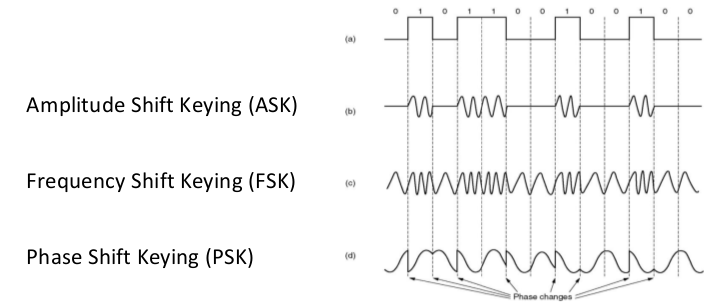
\includegraphics[width=0.8\linewidth]{img/phase.png}
    \end{center}

\end{itemize}
\end{itemize}

\subsection{GPRS core network}

GPRS introduces new nodes in the core network to support 
packet-switched data transfer:
\begin{figure}
	\centering
	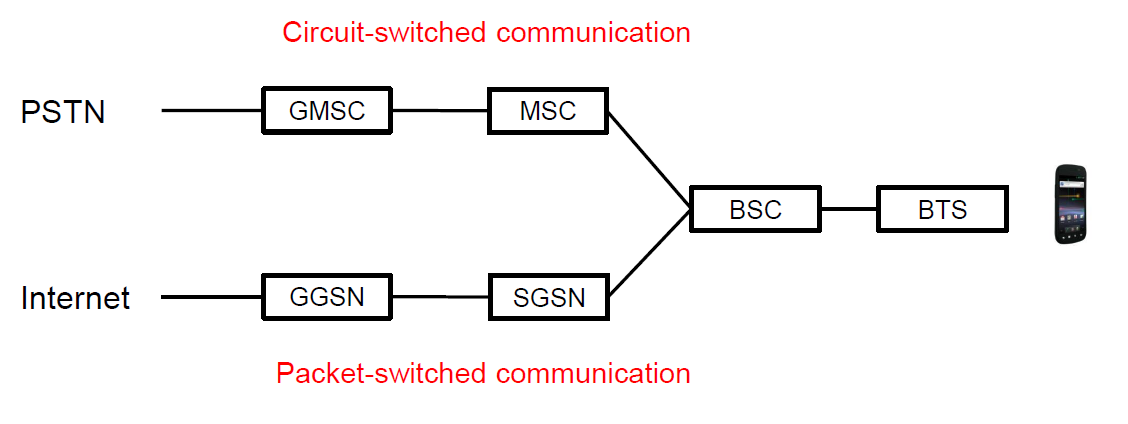
\includegraphics[scale=0.5]{img/gprs.png}
\end{figure}

\begin{description}
	\item[Gateway GPRS support node (GGSN):] Gateway to Internet
	\item[Serving GPRS support node (SGSN):] node between MSC and
	BS, does all the packet handling, routing, \ldots
\end{description}

\subsection{GPRS operation}
GPRS operation similar to GSM, phone connects to network, authenticates itself 
and request traffic channel. 

$\Rightarrow$ MS communicates with SGSN and GGSN (instead
of MSC and GMSC)

 \subsubsection{Encryption}
 Encryption is done \textbf{between the MS and SGSN} (instead of MS and BTS):
 \begin{itemize}
         \proitem{} More secure, since communication between BTS and BSC is often carried 
		over microwave links
		\proitem{} Better support for mobility: MS can smoothly move to a different cell 
		of the SGSN without too much overhead
        \consitem{} SGSN must have more processing power than BTS because it has 
		to encrypt/decrypt traffic for many MS
\end{itemize}

\subsubsection{Connection Management}
\begin{itemize}
	\item When opening a connection, PDP (Packet Data Protocol) context is
	created
	\item No dedicated channel resources allocared for PDP: MS can stay
	always ''connected'' to Internet wihtout using resources
	\item PDTCH only used when needed
\end{itemize}

In GSM, BSC allocates a physical channel for the TCH when initialing a
call and handover requires new TCH in target cell.

\subsubsection{IP traffic routing in GPRS}
Together with the PDP context, the GGSN allocates an IP address for the MS.
The traffic is transported over IP between the GGSN and the current SGSN of
the MS.

\paragraph{When MS roams to a new SGSN} $\Rightarrow$ Route change so the IP address
of the MS is changed + change routing table of all involved routers (Not suited!)

\paragraph{GPRS Tunneling Protocol (GPT)}
Protocol that runs on top of UDP:
\begin{itemize}
	\item GTP packet contains the IP adress of the MS
	\item UDP packet contains the address of the current SGSN
	\begin{itemize}
		\item Set by the GGSN when the traffic enters the GPRS network
		from the Internet
		\item GGSN is informed whenever the MS changes to a different
		SGSN
	\end{itemize}
\end{itemize}
When you have roamed to a different operator, your IP traffic is routed to the 
GGSN of your home operator

